%=======================================================================
%  IE 5311-001 (D01) Principles of Optimization
%  Homework 03 solutions
%
%  Packages: geometry, amsmath, amssymb, amsthm, booktabs, array,
%  graphicx. All ship with Overleaf and with a full TeX Live install.
%  The figure p1_cost_distributions.pdf must sit beside this file.
%=======================================================================
\documentclass[11pt]{article}

\usepackage[margin=1in]{geometry}
\usepackage{amsmath}
\usepackage{amssymb}
\usepackage{amsthm}
\usepackage{booktabs}
\usepackage{array}
\usepackage{graphicx}

\DeclareMathOperator*{\minimize}{min}
\DeclareMathOperator*{\maximize}{max}
\DeclareMathOperator{\CVaR}{CVaR}
\DeclareMathOperator{\VaR}{VaR}
\DeclareMathOperator{\spn}{span}
\DeclareMathOperator{\rank}{rank}

% Required by Problem 3.
\theoremstyle{definition}\newtheorem*{definition}{Definition}

\newtheorem{proposition}{Proposition}
\newtheorem{lemma}{Lemma}
\theoremstyle{definition}
\newtheorem{remark}{Remark}

\setlength{\parskip}{0.45em}
\setlength{\parindent}{0pt}

\begin{document}

\begin{center}
  {\large IE 5311-001 (D01) Principles of Optimization}\\[4pt]
  Lidivine Kengne\\[2pt]
  Homework 03
\end{center}
\vspace{0.6em}

%=======================================================================
\section*{Problem 1.\quad Emergency Relief Planning under Uncertainty
  \quad[35 pts]}
%=======================================================================

\subsection*{Sets}

\begin{center}
\begin{tabular}{@{}ll@{}}
\toprule
Symbol & Definition \\
\midrule
$I = \{1,2,3\}$ & Regional distribution centres, indexed by $i$ \\
$J = \{1,2,3,4\}$ & Demand regions, indexed by $j$ \\
$S = \{1,\dots,10\}$ & Disaster scenarios, indexed by $s$ \\
\bottomrule
\end{tabular}
\end{center}

\subsection*{Parameters}

\begin{center}
\begin{tabular}{@{}lll@{}}
\toprule
Symbol & Definition & Units \\
\midrule
$c_i$ & Pre-positioning cost per unit at centre $i$ & \$/unit \\
$\bar{x}_i$ & Storage capacity of centre $i$ & units \\
$B$ & Total pre-positioning budget, $B = 6000$ & \$ \\
$p_s$ & Probability of scenario $s$, $\sum_{s\in S} p_s = 1$ & --- \\
$d_{js}$ & Demand of region $j$ under scenario $s$ & units \\
$a_{is}$ & Fraction of inventory at centre $i$ accessible
  under scenario $s$ & --- \\
$q_{ij}$ & Shipping cost per unit from centre $i$ to region $j$
  & \$/unit \\
$\kappa_j$ & Penalty per unit of unmet demand at region $j$ & \$/unit \\
$w_j$ & Severity weight of region $j$ in the shortage loss & --- \\
$\theta$ & Required service fraction, $\theta = 0.90$ & --- \\
$\gamma$ & Required reliability of the chance constraint,
  $\gamma = 0.90$ & --- \\
$\alpha$ & CVaR confidence level, $\alpha = 0.90$ & --- \\
$\Lambda$ & Upper bound on the CVaR of the shortage loss,
  $\Lambda = 75$ & weighted units \\
\bottomrule
\end{tabular}
\end{center}

Three distinct quantities equal $0.90$ in this instance and are kept
apart on purpose: $\theta$ is the fraction of demand a region must
receive, $\gamma$ is the probability with which that must happen, and
$\alpha$ is the CVaR level.

\subsection*{Decision variables}

\emph{First stage}, chosen before the disaster is observed:
\[
  x_i \ge 0 \;=\; \text{units pre-positioned at centre } i
  \quad [\text{units}], \qquad i \in I .
\]
\emph{Second stage}, chosen after scenario $s$ is observed:
\[
  y_{ijs} \ge 0 \;=\; \text{units shipped from centre } i
  \text{ to region } j \text{ under scenario } s \quad [\text{units}],
\]
\[
  u_{js} \ge 0 \;=\; \text{unmet demand of region } j
  \text{ under scenario } s \quad [\text{units}].
\]
Every second-stage quantity carries the scenario index $s$: the shipping
plan is a recourse decision, not a here-and-now one.

%-----------------------------------------------------------------------
\subsection*{1.\quad The two-stage stochastic programming model}

\begin{align}
  \minimize_{x,\,y,\,u} \quad
    & \sum_{i \in I} c_i x_i
      \;+\; \sum_{s \in S} p_s \left[
        \sum_{i \in I}\sum_{j \in J} q_{ij}\, y_{ijs}
        \;+\; \sum_{j \in J} \kappa_j\, u_{js} \right]
      \label{eq:p1obj}\\
  \text{s.t.}\quad
    & \sum_{i \in I} c_i x_i \;\le\; B
      && \text{(budget)} \label{eq:budget}\\
    & 0 \;\le\; x_i \;\le\; \bar{x}_i
      && \forall\, i \in I \label{eq:cap}\\
    & \sum_{j \in J} y_{ijs} \;\le\; a_{is}\, x_i
      && \forall\, i \in I,\; s \in S \label{eq:avail}\\
    & \sum_{i \in I} y_{ijs} + u_{js} \;=\; d_{js}
      && \forall\, j \in J,\; s \in S \label{eq:bal}\\
    & y_{ijs} \ge 0,\quad u_{js} \ge 0
      && \forall\, i \in I,\; j \in J,\; s \in S .
\end{align}

The first-stage cost is deterministic; the bracketed term is the
scenario cost, and the objective is its expectation. Constraint
\eqref{eq:avail} is the only place the disaster touches supply: of the
$x_i$ units stored at centre $i$, only the fraction $a_{is}$ can be moved
once scenario $s$ has happened. Constraint \eqref{eq:bal} splits each
region's demand into what is delivered and what is not; together with
$y \ge 0$ and $u \ge 0$ it also records the bound
\begin{equation}
  0 \;\le\; u_{js} \;\le\; d_{js}
  \qquad \forall\, j \in J,\; s \in S,
  \label{eq:ubound}
\end{equation}
which is what makes the big-$M$ coefficients of Part 2 computable.

%-----------------------------------------------------------------------
\subsection*{2.\quad The joint chance constraint and its MILP form}

Region $j$ is adequately served under scenario $s$ exactly when it
receives at least the fraction $\theta$ of its demand, that is when
$\sum_i y_{ijs} \ge \theta d_{js}$, equivalently
$u_{js} \le (1-\theta) d_{js}$. The agency's requirement is that
\emph{all four} regions be adequately served, with probability at least
$\gamma$:
\begin{equation}
  \mathbb{P}\Big(
    u_{j}(x,\xi) \le (1-\theta)\, d_{j}(\xi)
    \;\; \forall\, j \in J \Big) \;\ge\; \gamma .
  \label{eq:joint}
\end{equation}

Under the finite scenario distribution this is a weighted count.
Introduce one binary per scenario,
\[
  z_s \in \{0,1\} \;=\;
  \begin{cases}
    1 & \text{if scenario $s$ is required to be adequately served},\\
    0 & \text{otherwise},
  \end{cases}
  \qquad s \in S,
\]
and write
\begin{align}
  & u_{js} \;\le\; (1-\theta)\, d_{js} \;+\; M_{js}\,(1 - z_s)
    && \forall\, j \in J,\; s \in S \label{eq:serve}\\
  & \sum_{s \in S} p_s\, z_s \;\ge\; \gamma \label{eq:count}\\
  & z_s \in \{0,1\} && \forall\, s \in S .
\end{align}
When $z_s = 1$ row \eqref{eq:serve} enforces the service level in
scenario $s$; when $z_s = 0$ it must be slack enough to impose nothing.
Row \eqref{eq:count} then says the scenarios that are served carry at
least probability $\gamma$, which is \eqref{eq:joint}.

\paragraph{Smallest valid big-$M$.} For $z_s = 0$ the row must not cut
off any otherwise feasible point, so it must hold at the largest value
$u_{js}$ can take. By \eqref{eq:ubound} that value is $d_{js}$, hence
\[
  (1-\theta)\,d_{js} + M_{js} \;\ge\; d_{js}
  \quad\Longleftrightarrow\quad
  M_{js} \;\ge\; \theta\, d_{js},
\]
and the smallest valid coefficient is
\begin{equation}
  \boxed{\;M_{js} = \theta\, d_{js} = 0.9\, d_{js}\;}
  \qquad \forall\, j \in J,\; s \in S .
  \label{eq:M}
\end{equation}
It depends on both the region and the scenario, which is the point of the
hint: a single global $M = \theta \max_{j,s} d_{js} = 76.5$ would be
valid but needlessly loose on every row except one, weakening the linear
relaxation. The $40$ coefficients range from $M_{1,1} = 27$ to
$M_{3,10} = 76.5$.

%-----------------------------------------------------------------------
\subsection*{3.\quad Individual chance constraints are not equivalent}

Write $A_j := \{\, \xi :\; u_j(x,\xi) \le (1-\theta) d_j(\xi) \,\}$ for
the event that region $j$ is adequately served. The joint requirement is
$\mathbb{P}\big(\bigcap_{j \in J} A_j\big) \ge \gamma$; the individual
requirements are $\mathbb{P}(A_j) \ge \gamma$ for every $j \in J$. They
are \textbf{not} equivalent: the joint constraint is strictly stronger.

\paragraph{Joint implies individual.} For each $j$ we have
$\bigcap_{k \in J} A_k \subseteq A_j$, so by monotonicity of probability
\[
  \mathbb{P}(A_j) \;\ge\;
  \mathbb{P}\Big(\bigcap_{k \in J} A_k\Big) \;\ge\; \gamma .
\]

\paragraph{Individual does not imply joint.} Suppose only that
$\mathbb{P}(A_j) \ge \gamma$ for every $j$. By De Morgan and the union
bound,
\begin{equation}
  \mathbb{P}\Big(\bigcap_{j \in J} A_j\Big)
  = 1 - \mathbb{P}\Big(\bigcup_{j \in J} A_j^{c}\Big)
  \;\ge\; 1 - \sum_{j \in J} \mathbb{P}(A_j^{c})
  \;\ge\; 1 - |J|\,(1-\gamma)
  = 1 - 4(0.10) = 0.60 ,
  \label{eq:bonferroni}
\end{equation}
and $0.60$ is all that can be guaranteed. The bound is attained, so no
better one exists: it is tight exactly when the four failure events are
disjoint and each has probability $1-\gamma$.

\paragraph{A counterexample in this instance.} The data admit one
directly. Scenarios $2,3,4,5$ each carry $p_s = 0.10$. Suppose a plan
fails region $1$ only in scenario $2$, region $2$ only in scenario $3$,
region $3$ only in scenario $4$ and region $4$ only in scenario $5$, and
serves every region in every other scenario. Then
$\mathbb{P}(A_j^{c}) = 0.10$, so $\mathbb{P}(A_j) = 0.90 = \gamma$ for
each $j$ and all four individual constraints hold. But the four failures
are disjoint, so
\[
  \mathbb{P}\Big(\bigcap_{j\in J} A_j\Big)
  = 1 - (0.10 + 0.10 + 0.10 + 0.10) = 0.60 \;<\; 0.90 = \gamma,
\]
and the joint constraint fails. Hence the individual system admits plans
the joint system rejects: its feasible region is a strict superset.

\begin{remark}
The two coincide only in degenerate cases, for instance when the failure
events are nested, or when $|J| = 1$. In general, to guarantee a joint
reliability of $\gamma$ through individual constraints one must impose
them at the Bonferroni level $1 - (1-\gamma)/|J| = 0.975$ per region,
which is conservative in the opposite direction.
\end{remark}

%-----------------------------------------------------------------------
\subsection*{4.\quad The CVaR constraint}

The system shortage loss under scenario $s$ is
$L_s = \sum_{j \in J} w_j u_{js}$, and the requirement is
$\CVaR_{\alpha}(L) \le \Lambda$ with
\[
  \CVaR_{\alpha}(L) \;:=\;
  \inf_{\eta \in \mathbb{R}}
  \left\{ \eta + \frac{1}{1-\alpha}\,
    \mathbb{E}\big[(L-\eta)^{+}\big] \right\} .
\]

Because $\CVaR_\alpha$ is defined as an \emph{infimum} and the
requirement is an \emph{upper} bound, the constraint holds if and only if
\emph{some} $\eta$ achieves the bound. So $\eta$ may be introduced as a
free decision variable rather than fixed at $\VaR_\alpha$, and no
separate inner minimisation is needed. With $v_s$ modelling
$(L_s - \eta)^{+}$ over the finite support,
\begin{align}
  & \eta \;+\; \frac{1}{1-\alpha}
      \sum_{s \in S} p_s\, v_s \;\le\; \Lambda \label{eq:cvar}\\
  & v_s \;\ge\; \sum_{j \in J} w_j\, u_{js} \;-\; \eta
    && \forall\, s \in S \label{eq:cvarepi}\\
  & v_s \;\ge\; 0 \quad \forall\, s \in S,
    \qquad \eta \in \mathbb{R} .
\end{align}
Rows \eqref{eq:cvarepi} and $v_s \ge 0$ together give
$v_s \ge (L_s - \eta)^{+}$, and since $v_s$ appears with a positive
coefficient on the left of \eqref{eq:cvar}, which is being bounded above,
the inequality is tight at any solution that satisfies it. The
reformulation is therefore exact.

%-----------------------------------------------------------------------
\subsection*{5.\quad The complete model}

\begin{align}
  \minimize_{x,y,u,z,\eta,v} \quad
    & \sum_{i \in I} c_i x_i
      + \sum_{s \in S} p_s \left[
        \sum_{i \in I}\sum_{j \in J} q_{ij} y_{ijs}
        + \sum_{j \in J} \kappa_j u_{js} \right] \\
  \text{s.t.}\quad
    & \sum_{i \in I} c_i x_i \le B,
      \qquad 0 \le x_i \le \bar{x}_i
      && \forall\, i \in I \\
    & \sum_{j \in J} y_{ijs} \le a_{is} x_i
      && \forall\, i \in I,\; s \in S \\
    & \sum_{i \in I} y_{ijs} + u_{js} = d_{js}
      && \forall\, j \in J,\; s \in S \\
    & u_{js} \le (1-\theta) d_{js} + \theta d_{js}\,(1-z_s)
      && \forall\, j \in J,\; s \in S \\
    & \sum_{s \in S} p_s z_s \ge \gamma \\
    & v_s \ge \sum_{j \in J} w_j u_{js} - \eta
      && \forall\, s \in S \\
    & \eta + \frac{1}{1-\alpha}\sum_{s \in S} p_s v_s \le \Lambda \\
    & y_{ijs} \ge 0,\; u_{js} \ge 0,\; v_s \ge 0,\;
      z_s \in \{0,1\},\; \eta \in \mathbb{R}
      && \forall\, i \in I,\, j \in J,\, s \in S .
\end{align}

\paragraph{Classification (taxonomy, slides 8--10).}

\begin{center}
\begin{tabular}{@{}ll@{}}
\toprule
Question & Answer \\
\midrule
Constrained? & Yes \\
Variable type and size & Mixed integer: $174$ continuous
  ($|I| + |I||J||S| + |J||S| + 1 + |S|$) and $|S| = 10$ binary \\
Objective type & Linear \\
Constraint type and size & Linear, $123$ rows \\
Parameters & Stochastic, finite support, probabilities $p_s$ known \\
Stages and players & Two stages, one player \\
\bottomrule
\end{tabular}
\end{center}

Dropping rows \eqref{eq:serve}--\eqref{eq:count} and
\eqref{eq:cvar}--\eqref{eq:cvarepi} gives the risk-neutral model, which
is a pure linear program with $163$ variables and $71$ rows; the binaries
enter only with the chance constraint.

%-----------------------------------------------------------------------
\subsection*{6.\quad Solutions of the three models}

Solved with Gurobi. All three are feasible and solve to proven
optimality.

\begin{center}
\begin{tabular}{@{}lrrrr@{}}
\toprule
Model & Objective & $x_1$ & $x_2$ & $x_3$ \\
\midrule
Risk neutral          & $6481.4607$ & $94.2857$ & $35.0000$ & $110.0000$ \\
Chance constrained    & $6800.4958$ & $70.8333$ & $100.0000$ & $110.0000$ \\
Chance $+$ CVaR       & $7064.0235$ & $94.8529$ & $100.0000$ & $110.0000$ \\
\bottomrule
\end{tabular}
\end{center}

\begin{center}
\begin{tabular}{@{}lrrr@{}}
\toprule
Model & Spend & Units stored & Size \\
\midrule
Risk neutral       & $4522.14$ & $239.29$ & $163$ vars, $71$ rows \\
Chance constrained & $5465.00$ & $280.83$ & $173$ vars (10 binary),
  $112$ rows \\
Chance $+$ CVaR    & $5897.35$ & $304.85$ & $184$ vars (10 binary),
  $123$ rows \\
\bottomrule
\end{tabular}
\end{center}

Three things are worth reading off these numbers.

\emph{Risk management is bought with inventory.} The budget is \$6000 and
filling every centre to capacity would cost
$\sum_i c_i \bar{x}_i = 6350$, so the budget binds before capacity does.
The risk-neutral plan spends only $4522$ of it: beyond that point extra
inventory costs more than the expected penalty it avoids. Adding the
chance constraint pushes the spend to $5465$ and adding CVaR to $5897$,
nearly the whole budget.

\emph{Which scenarios are sacrificed.} In both constrained models the
binaries come back $z_s = 1$ for $s = 1,\dots,9$ and $z_{10} = 0$, so
scenario $10$ is the one left unserved, at probability
$p_{10} = 0.08 \le 1-\gamma = 0.10$. That is forced rather than chosen.
Scenario $10$ has total demand
$\sum_j d_{j,10} = 310$ and accessibility $(a_{1,10}, a_{2,10}, a_{3,10})
= (0.70, 0.70, 0.75)$, so even filling every centre to capacity and
ignoring the budget leaves only
\[
  \sum_{i \in I} a_{i,10}\,\bar{x}_i
  = 0.70(120) + 0.70(100) + 0.75(110) = 236.5
\]
units reachable, against the $0.90 \times 310 = 279$ that $90\%$ service
in all four regions requires. It is capacity, not budget, that rules
scenario $10$ out, so $z_{10} = 0$ in every feasible solution. Every other single scenario carries probability at least $0.10$,
and no two scenarios can be dropped together, since the smallest pair
sums to $0.18 > 0.10$. So the chance constraint is feasible, and it is
feasible in exactly one way.

\emph{The CVaR constraint binds.} At the optimum of the third model
$\eta = 10.5882$ and $\CVaR_{0.90}(L) = 75.0000$, exactly at the cap
$\Lambda$. It is an active constraint, not a formality, which is why the
first-stage plan moves again between the second and third models.

%-----------------------------------------------------------------------
\subsection*{7.\quad Out-of-sample evaluation on 5{,}000 draws}

Five thousand scenario indices were drawn independently from
$(p_1,\dots,p_{10})$. For each of the three first-stage plans and each
realised scenario the operator ships at minimum realised cost, so the
evaluation solves the recourse problem
\[
  \minimize_{y,u \ge 0}\;
  \sum_{i \in I}\sum_{j \in J} q_{ij} y_{ij}
  + \sum_{j \in J} \kappa_j u_j
  \quad\text{s.t.}\quad
  \sum_{j} y_{ij} \le a_{is} x_i,\;\;
  \sum_{i} y_{ij} + u_j = d_{js},
\]
and reports $\sum_i c_i x_i$ plus that value. Since the support has only
ten atoms, this is thirty linear programs; the sample then indexes into
them.

\begin{center}
\begin{tabular}{@{}lrrrrrr@{}}
\toprule
Model & $\mathbb{E}[\text{cost}]$ & s.d. & $90\%$ quantile &
  $\CVaR_{0.90}$ & max & $\CVaR_{0.90}(L)$ \\
\midrule
Risk neutral       & $6416.66$ & $1958.39$ & $8870.50$ & $11289.81$
  & $11894.64$ & $124.79$ \\
Chance constrained & $6748.95$ & $1399.26$ & $7502.50$ & $10601.17$
  & $11375.83$ & $91.33$ \\
Chance $+$ CVaR    & $7037.13$ & $1188.27$ & $7343.97$ & $10323.50$
  & $11068.38$ & $75.00$ \\
\bottomrule
\end{tabular}
\end{center}

\begin{figure}[htbp]
\centering
% Figure source, tried in order:
%   1. p1_cost_excel.pdf  - the Excel chart exported to PDF (preferred)
%   2. p1_cost_excel.png  - the Excel chart saved as a picture
%   3. p1_cost_distributions.pdf - the matplotlib fallback
% All three are built from the same numbers.
\IfFileExists{p1_cost_excel.pdf}
  {\includegraphics[width=0.92\textwidth]{p1_cost_excel.pdf}}
  {\IfFileExists{p1_cost_excel.png}
    {\includegraphics[width=0.92\textwidth]{p1_cost_excel.png}}
    {\IfFileExists{p1_cost_distributions.pdf}
      {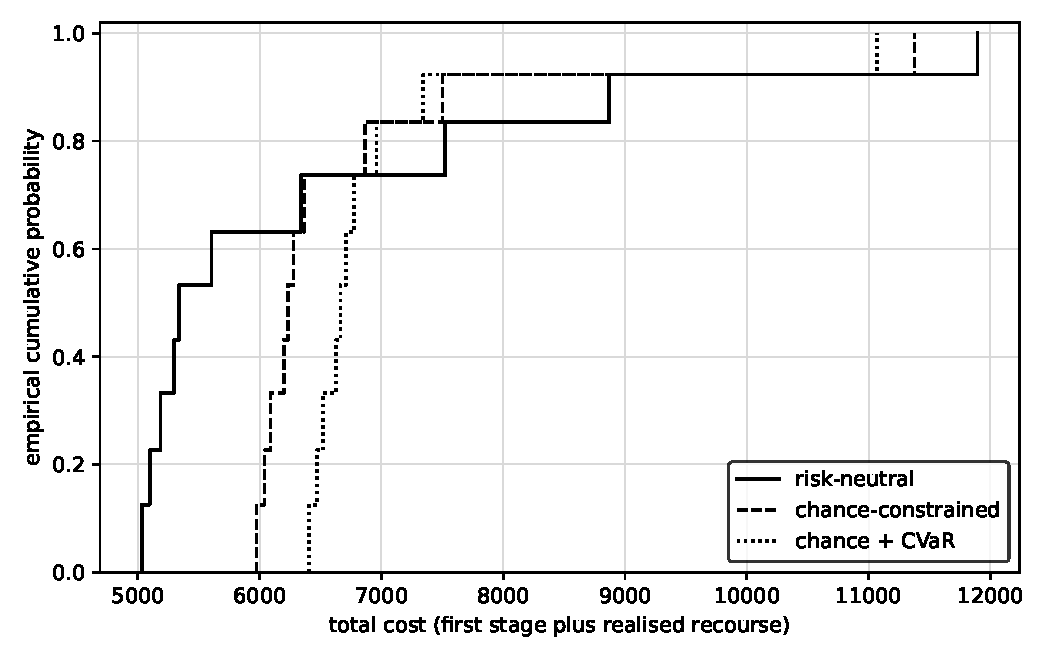
\includegraphics[width=0.84\textwidth]{p1_cost_distributions.pdf}}
      {\fbox{\parbox{0.8\textwidth}{\centering \vspace{1em}
       No figure file found. Export the \texttt{Figure} sheet of
       \texttt{p1\_cost\_distributions.xlsx} as
       \texttt{p1\_cost\_excel.pdf}, or run \texttt{p1\_relief.py}
       for the fallback. \vspace{1em}}}}}}
\caption{Empirical distribution of total cost over $5{,}000$ draws, for
the three first-stage plans. The support has ten atoms, so each curve is
a staircase whose risers sit at the per-scenario costs of Part 6. Moving
from the solid curve to the dashed and dotted ones shifts mass to the
right in the body of the distribution and pulls the rightmost riser to the
left: the constrained plans cost more most of the time and less in the
worst case, which is the trade the chance and CVaR constraints exist to
make. Built in \texttt{p1\_cost\_distributions.xlsx}, sheet
\texttt{Figure}, from the step-expanded cumulative frequencies on its
\texttt{ChartData} sheet.}
\end{figure}

\paragraph{Expected performance.} The ordering is monotone and is the
price of protection: $6416.66 < 6748.95 < 7037.13$. The chance constraint
costs about $5.2\%$ of expected cost and the CVaR constraint a further
$4.3\%$. The sample means sit below the model objectives
($6481.46$, $6800.50$, $7064.02$), and the gap has two distinct parts
that are worth separating.

\begin{center}
\begin{tabular}{@{}lrrrrr@{}}
\toprule
Model & Objective & $\mathbb{E}$ under free & Recourse
  & Sample mean & Sampling \\
 & & recourse & relaxation & & noise \\
\midrule
Risk neutral       & $6481.4607$ & $6481.4607$ & $0.0000$
  & $6416.66$ & $64.80$ \\
Chance constrained & $6800.4958$ & $6783.9833$ & $16.5125$
  & $6748.95$ & $35.03$ \\
Chance $+$ CVaR    & $7064.0235$ & $7062.3471$ & $1.6765$
  & $7037.13$ & $25.22$ \\
\bottomrule
\end{tabular}
\end{center}

The risk-neutral model already minimises expected cost with free
recourse, so its objective equals the exact expectation to the last
digit and its entire gap to the sample mean is sampling noise. Scenario
$8$ drew at frequency $0.089$ against $p_8 = 0.10$ and is the second most
expensive atom, which accounts for most of that $64.80$.

The two constrained models carry a second gap that is systematic rather
than statistical. Their objectives price the recourse the model itself
plans, which must respect the service rows in scenarios $1$ through $9$
and the CVaR cap. The evaluation drops both and lets the operator
minimise realised cost, which is weakly cheaper, so the exact
expectation falls below the objective by $16.51$ and $1.68$
respectively. That relaxation is not an artefact of the sample; it is
the same effect as the service-adequacy gap reported below, seen on the
cost side instead of the service side.

\paragraph{Tail behaviour.} The tail moves in the opposite direction to
the mean, which is the whole point of the exercise. The standard
deviation falls by $39\%$ from $1958$ to $1188$; the $90\%$ quantile
falls by $17\%$ from $8870.50$ to $7343.97$; $\CVaR_{0.90}$ of total cost
falls from $11289.81$ to $10323.50$; the worst realisation falls from
$11894.64$ to $11068.38$. The constrained plans give up roughly $620$ in
expectation to remove roughly $966$ from the conditional tail average.
The shortage loss shows the same pattern more sharply, with
$\CVaR_{0.90}(L)$ falling from $124.79$ to exactly the imposed cap of
$75$.

\paragraph{A gap worth reporting.} Service adequacy, measured as the
probability that all four regions receive at least $90\%$ of demand,
behaves differently depending on who is asked:

\begin{center}
\begin{tabular}{@{}lrr@{}}
\toprule
Model & Planned by the model & Realised under cost-minimising recourse \\
\midrule
Risk neutral       & $0.62$ & $0.62$ \\
Chance constrained & $0.92$ & $0.72$ \\
Chance $+$ CVaR    & $0.92$ & $0.82$ \\
\bottomrule
\end{tabular}
\end{center}

The chance constraint is satisfied inside the model: its own
second-stage solution serves scenarios $1$ through $9$, probability
$0.92 \ge \gamma$. But the constraint only guarantees that a recourse
achieving $90\%$ service \emph{exists} with probability $\gamma$. If the
operator afterwards minimises realised cost scenario by scenario, which
is what the evaluation assumes, paying the penalty $\kappa_j$ can be
cheaper than shipping, and the realised rate drops to $0.72$. The CVaR
constraint closes part of that gap, to $0.82$, because it prices
shortages a second time through $L$ and so makes shipping worthwhile in
more cases.

This is not a defect of the formulation; it is a statement about what a
chance constraint on a two-stage program actually promises. If the agency
wants the service level to hold in operation and not merely in the plan,
the service rows must be imposed on the executed policy as well, for
example by writing them into the operating rule or by raising $\kappa_j$
until the cost-minimising recourse delivers them on its own.

%=======================================================================
\newpage
\section*{Problem 2.\quad Indicator Variable Reformulation \quad[25 pts]}
%=======================================================================

Throughout, $x \in \mathbb{R}^n$ satisfies the box bounds
$\ell \le x \le u$ componentwise, and $z_k \in \{0,1\}$ for $k \in K$.
Two quantities are used repeatedly, and both are written out rather than
named:
\begin{equation}
  \overline{V}(a) \;:=\; \maximize_{\ell \le x \le u} a^{\!\top} x
  \;=\; \sum_{i=1}^{n} \max\{\, a_i \ell_i,\; a_i u_i \,\},
  \qquad
  \underline{V}(a) \;:=\; \minimize_{\ell \le x \le u} a^{\!\top} x
  \;=\; \sum_{i=1}^{n} \min\{\, a_i \ell_i,\; a_i u_i \,\} .
  \label{eq:VV}
\end{equation}
Both are separable because the box is a product of intervals and
$a^{\!\top}x$ is separable, and each is attained at a vertex of the box:
$\overline{V}(a)$ at $x_i = u_i$ when $a_i \ge 0$ and $x_i = \ell_i$
otherwise, and $\underline{V}(a)$ at the opposite corner.

%-----------------------------------------------------------------------
\subsection*{1.\quad Big-$M$ reformulation of the two implications}

For $k \in K_1$ the requirement is
$z_k = 1 \Rightarrow a_k^{\!\top} x \le b_k$. Relax the row by an amount
that is zero when $z_k = 1$:
\begin{equation}
  a_k^{\!\top} x \;\le\; b_k + M_k\,(1 - z_k)
  \qquad \forall\, k \in K_1 .
  \label{eq:k1}
\end{equation}
For $k \in K_2$ the requirement is
$z_k = 0 \Rightarrow a_k^{\!\top} x \ge b_k$, so the relaxation must
switch on when $z_k = 1$:
\begin{equation}
  a_k^{\!\top} x \;\ge\; b_k - N_k\, z_k
  \qquad \forall\, k \in K_2 .
  \label{eq:k2}
\end{equation}
In each case the implication is reproduced when the binary takes the
triggering value, and the row must be redundant otherwise.

%-----------------------------------------------------------------------
\subsection*{2.\quad The smallest valid coefficients}

\begin{proposition}
Using only $\ell \le x \le u$, the smallest valid coefficients in
\eqref{eq:k1} and \eqref{eq:k2} are
\[
  M_k = \max\big\{0,\; \overline{V}(a_k) - b_k \big\},
  \qquad
  N_k = \max\big\{0,\; b_k - \underline{V}(a_k) \big\} .
\]
\end{proposition}

\begin{proof}
Take \eqref{eq:k1}. At $z_k = 0$ the row reads
$a_k^{\!\top}x \le b_k + M_k$, and it must not exclude any $x$ in the
box. The largest value of the left side over the box is
$\overline{V}(a_k)$, so redundancy is equivalent to
$\overline{V}(a_k) \le b_k + M_k$, that is
$M_k \ge \overline{V}(a_k) - b_k$. Combined with $M_k \ge 0$, the
smallest admissible value is the stated maximum.

Smallest means no valid coefficient is smaller. If
$\overline{V}(a_k) \le b_k$ then $M_k = 0$ and nothing smaller is
admissible, since a negative coefficient would tighten the row at
$z_k = 0$ instead of relaxing it. If $\overline{V}(a_k) > b_k$ then
$M_k = \overline{V}(a_k) - b_k > 0$, and for any
$M' < M_k$ the box corner $x^{\star}$ with $x^{\star}_i = u_i$ when
$a_{ki} \ge 0$ and $x^{\star}_i = \ell_i$ otherwise satisfies
\[
  a_k^{\!\top} x^{\star} = \overline{V}(a_k) = b_k + M_k > b_k + M',
\]
so the row with coefficient $M'$ excludes $x^{\star}$ at $z_k = 0$ and is
not valid. The argument for \eqref{eq:k2} is the same with the minimum in
place of the maximum and the inequality reversed.
\end{proof}

Both bounds were checked numerically on $4{,}000$ random instances each:
the stated coefficient is valid every time, and reducing it by
$10^{-6}$ cuts off a feasible box point every time, so it is not merely
valid but tight.

%-----------------------------------------------------------------------
\subsection*{3.\quad The pairwise implication, without a new binary}

The requirement is
$z_k = z_\ell = 1 \Rightarrow c_{k\ell}^{\!\top} x \le d_{k\ell}$ for
$(k,\ell) \in E$. Use the quantity $2 - z_k - z_\ell$, which is $0$
exactly when both binaries are $1$ and at least $1$ otherwise:
\begin{equation}
  c_{k\ell}^{\!\top} x \;\le\;
  d_{k\ell} + M_{k\ell}\,\big(2 - z_k - z_\ell\big)
  \qquad \forall\, (k,\ell) \in E .
  \label{eq:pair}
\end{equation}
No auxiliary binary is introduced; the product $z_k z_\ell$ is avoided
because only the implication in one direction is required, and the
linear expression $2 - z_k - z_\ell$ separates that one case from the
other three.

\begin{proposition}
The smallest valid coefficient in \eqref{eq:pair} is
$M_{k\ell} = \max\{0,\; \overline{V}(c_{k\ell}) - d_{k\ell}\}$.
\end{proposition}

\begin{proof}
Three patterns must leave the row redundant. If exactly one of
$z_k, z_\ell$ equals $1$ the multiplier is $1$ and the row reads
$c_{k\ell}^{\!\top}x \le d_{k\ell} + M_{k\ell}$, which by the argument of
Part 2 requires exactly $M_{k\ell} \ge \overline{V}(c_{k\ell}) -
d_{k\ell}$. If both are $0$ the multiplier is $2$ and the right side is
larger still, so that case imposes nothing further. The binding pattern
is therefore the single-active one, and the stated value is smallest.
\end{proof}

%-----------------------------------------------------------------------
\subsection*{4.\quad Violation permitted only under an active condition}

The requirement is that $g_r^{\!\top} x > h_r$ be permitted only if
$\sum_{k \in K_r} z_k \ge 1$. Its contrapositive is the implementable
form: if no condition in $K_r$ is active then the row must hold. Since
$\sum_{k\in K_r} z_k$ is a nonnegative integer that is $0$ exactly when
none is active,
\begin{equation}
  g_r^{\!\top} x \;\le\; h_r
    + M_r \sum_{k \in K_r} z_k
  \qquad \forall\, r \in R,
  \qquad
  M_r = \max\big\{0,\; \overline{V}(g_r) - h_r \big\} .
  \label{eq:cover}
\end{equation}
At $\sum_k z_k = 0$ the row is exactly $g_r^{\!\top}x \le h_r$; at
$\sum_k z_k \ge 1$ it is relaxed by at least $M_r$ and so imposes
nothing. Note that this is a one-way implication only: it permits
violation when a condition is active but does not require it.

%-----------------------------------------------------------------------
\subsection*{5.\quad The logical equivalence}

Now both directions are required,
\[
  g_r^{\!\top} x > h_r
  \quad\Longleftrightarrow\quad
  \sum_{k \in K_r} z_k \ge 1 .
\]
The forward direction is \eqref{eq:cover}. The reverse direction,
$\sum_{k} z_k \ge 1 \Rightarrow g_r^{\!\top} x > h_r$, is equivalent to
requiring the implication for each $k$ separately, since the hypothesis
holds exactly when at least one $z_k$ equals $1$. A strict inequality
cannot be imposed directly, so introduce a tolerance $\epsilon > 0$ and
require $g_r^{\!\top} x \ge h_r + \epsilon$ instead:
\begin{align}
  & g_r^{\!\top} x \;\le\; h_r + M_r \sum_{k \in K_r} z_k
    && \forall\, r \in R \\
  & g_r^{\!\top} x \;\ge\; h_r + \epsilon - N_r\,(1 - z_k)
    && \forall\, r \in R,\; k \in K_r
  \label{eq:rev}
\end{align}
with $M_r$ as in \eqref{eq:cover} and, by the argument of Part 2 applied
to the reversed inequality,
\[
  N_r = \max\big\{0,\; h_r + \epsilon - \underline{V}(g_r) \big\} .
\]
Writing \eqref{eq:rev} once per $k \in K_r$ avoids any new binary: if
some $z_k = 1$ that row forces $g_r^{\!\top}x \ge h_r + \epsilon$, and if
every $z_k = 0$ all the rows are slack.

\paragraph{Why the tolerance cannot be removed.} On the branch
$\sum_k z_k \ge 1$ the exact condition demands
$g_r^{\!\top} x > h_r$, an open half-space. Take any $\bar{x}$ with
$g_r^{\!\top}\bar{x} = h_r$ and a sequence
$x^{(m)} \to \bar{x}$ with $g_r^{\!\top} x^{(m)} = h_r + 10^{-m}$. Every
$x^{(m)}$ satisfies the condition and the limit does not, so that branch
of the feasible set is not closed. The feasible set of a mixed-integer
linear program is a finite union of closed polyhedra and is therefore
closed. No exact MILP representation exists, and the formulation above
instead declares the band $(h_r,\, h_r + \epsilon)$ infeasible whenever a
condition is active. That band is the entire approximation, and it
shrinks to nothing as $\epsilon \downarrow 0$ without ever vanishing.

%=======================================================================
\newpage
\section*{Problem 3.\quad Linear Independence \quad[15 pts]}
%=======================================================================

Throughout, $V$ is a vector space over a field $\mathbb{F}$ and
$v_1,\dots,v_m \in V$ is a finite collection of vectors. The convention
$\spn(\emptyset) = \{0\}$ is used, so that the statements below behave
correctly when $m = 1$.

%-----------------------------------------------------------------------
\subsection*{1.\quad First definition}

\begin{definition}[no vector lies in the span of the others]
The collection $v_1,\dots,v_m$ is \emph{linearly independent} if for
every $i \in \{1,\dots,m\}$,
\[
  v_i \;\notin\; \spn\big(\{\, v_j :\; j \ne i \,\}\big),
\]
that is, no $v_i$ can be written as
$v_i = \sum_{j \ne i} \beta_j v_j$ with $\beta_j \in \mathbb{F}$.
\end{definition}

%-----------------------------------------------------------------------
\subsection*{2.\quad Second definition}

\begin{definition}[only the trivial combination vanishes]
The collection $v_1,\dots,v_m$ is \emph{linearly independent} if for all
scalars $\alpha_1,\dots,\alpha_m \in \mathbb{F}$,
\[
  \sum_{i=1}^{m} \alpha_i v_i = 0
  \quad\Longrightarrow\quad
  \alpha_1 = \alpha_2 = \dots = \alpha_m = 0 .
\]
\end{definition}

%-----------------------------------------------------------------------
\subsection*{3.\quad The two definitions are equivalent}

\begin{proof}
Both directions are shown by contraposition.

\emph{Definition 2 implies Definition 1.} Suppose Definition 1 fails.
Then there is an index $i$ with
$v_i \in \spn(\{v_j : j \ne i\})$, so there are scalars $\beta_j$ with
\[
  v_i = \sum_{j \ne i} \beta_j v_j .
\]
Rearranging gives
\[
  \sum_{j \ne i} \beta_j v_j \;+\; (-1)\, v_i \;=\; 0,
\]
a linear combination of $v_1,\dots,v_m$ equal to zero whose coefficient
on $v_i$ is $-1 \ne 0$. Hence Definition 2 fails.

\emph{Definition 1 implies Definition 2.} Suppose Definition 2 fails.
Then there are scalars $\alpha_1,\dots,\alpha_m$, not all zero, with
$\sum_{i=1}^{m} \alpha_i v_i = 0$. Choose an index $k$ with
$\alpha_k \ne 0$. Since $\mathbb{F}$ is a field, $\alpha_k$ is
invertible, and solving for $v_k$ gives
\[
  v_k \;=\; -\,\frac{1}{\alpha_k} \sum_{j \ne k} \alpha_j v_j
  \;\in\; \spn\big(\{\, v_j :\; j \ne k \,\}\big) .
\]
Hence Definition 1 fails.

Each definition therefore fails exactly when the other does, so they
hold in exactly the same cases and are equivalent.
\end{proof}

\begin{remark}
The convention $\spn(\emptyset) = \{0\}$ is what makes the case $m = 1$
work. Definition 1 then reads $v_1 \notin \{0\}$, that is $v_1 \ne 0$,
and Definition 2 reads $\alpha v_1 = 0 \Rightarrow \alpha = 0$, which for
a single vector is also exactly $v_1 \ne 0$. Invertibility of $\alpha_k$
is the only place the field structure is used; over a ring the second
direction can fail.
\end{remark}

%=======================================================================
\newpage
\section*{Problem 4.\quad Groups \quad[20 pts]}
%=======================================================================

%-----------------------------------------------------------------------
\subsection*{1.\quad The invertible $n \times n$ real matrices}

Let $G := \{\, A \in \mathbb{R}^{n \times n} :\; \det A \ne 0 \,\}$,
with the operation matrix multiplication.

\emph{Closure.} For $A, B \in G$ the product satisfies
$\det(AB) = \det(A)\det(B) \ne 0$, so $AB \in G$ and multiplication is
indeed a map $G \times G \to G$. Explicitly $(AB)^{-1} = B^{-1}A^{-1}$.

\emph{Associativity.} For any conformable matrices,
$\big((AB)C\big)_{ik} = \sum_{j,\ell} A_{i\ell} B_{\ell j} C_{jk}
= \big(A(BC)\big)_{ik}$, the two orders of summation agreeing because
addition and multiplication in $\mathbb{R}$ are associative,
commutative and distributive. Hence $(AB)C = A(BC)$.

\emph{Identity.} The matrix $I_n$ satisfies $I_n A = A I_n = A$ for every
$A$, and $\det I_n = 1 \ne 0$, so $I_n \in G$.

\emph{Inverse.} For $A \in G$ the matrix $A^{-1}$ exists because
$\det A \ne 0$, and satisfies $A A^{-1} = A^{-1} A = I_n$. It lies in
$G$, since $\det(A^{-1}) = 1/\det(A) \ne 0$.

All three group properties hold, so $G$ is a group. It is not abelian
for $n \ge 2$: with
$A = \left(\begin{smallmatrix}1&1\\0&1\end{smallmatrix}\right)$ and
$B = \left(\begin{smallmatrix}1&0\\1&1\end{smallmatrix}\right)$ one has
$AB \ne BA$. Commutativity is not required.

%-----------------------------------------------------------------------
\subsection*{2.\quad The rotations of a square}

Let $a, b, c, d$ denote the rotations by $0^{\circ}$, $90^{\circ}$,
$180^{\circ}$ and $270^{\circ}$ about the centre, with $xy$ meaning
``apply $y$ first, then $x$''. Writing $\tau(a) = 0$, $\tau(b) = 1$,
$\tau(c) = 2$, $\tau(d) = 3$ for the number of quarter turns, composition
adds quarter turns modulo $4$:
\begin{equation}
  \tau(xy) \;=\; \big(\tau(x) + \tau(y)\big) \bmod 4 .
  \label{eq:rot}
\end{equation}
This is the Cayley table:

\begin{center}
\begin{tabular}{@{}c|cccc@{}}
\toprule
 & $a$ & $b$ & $c$ & $d$ \\
\midrule
$a$ & $a$ & $b$ & $c$ & $d$ \\
$b$ & $b$ & $c$ & $d$ & $a$ \\
$c$ & $c$ & $d$ & $a$ & $b$ \\
$d$ & $d$ & $a$ & $b$ & $c$ \\
\bottomrule
\end{tabular}
\end{center}

\emph{Closure.} Every entry of the table lies in $\{a,b,c,d\}$, since
\eqref{eq:rot} returns a residue in $\{0,1,2,3\}$.

\emph{Associativity.} These are functions on the square and the operation
is composition of functions, which is associative. Equivalently, by
\eqref{eq:rot},
$\tau\big((xy)z\big) = (\tau(x)+\tau(y)+\tau(z)) \bmod 4
= \tau\big(x(yz)\big)$, using associativity of addition modulo $4$.

\emph{Identity.} The element $a$, the rotation by $0^{\circ}$, satisfies
$ax = xa = x$ for all $x$: its row and column reproduce the headings.

\emph{Inverse.} From the table, $aa = a$, $bd = db = a$, $cc = a$, so
\[
  a^{-1} = a, \qquad b^{-1} = d, \qquad c^{-1} = c, \qquad d^{-1} = b,
\]
and every element has one. Hence $\{a,b,c,d\}$ is a group. It is in fact
cyclic of order four, generated by $b$, since
$b, b^2 = c, b^3 = d, b^4 = a$ exhaust the set; it is also abelian,
the table being symmetric, though neither property was required.

%-----------------------------------------------------------------------
\subsection*{3.\quad The inverse of an element is unique}

\begin{proposition}
Let $(V,\cdot)$ be a group with identity $e$ and let $a \in V$. If
$b, c \in V$ both satisfy $ab = ba = e$ and $ac = ca = e$, then $b = c$.
\end{proposition}

\begin{proof}
Compute
\[
  b \;=\; b\,e \;=\; b\,(ac) \;=\; (ba)\,c \;=\; e\,c \;=\; c .
\]
The five steps use, in order: the identity property applied to $b$; the
inverse property of $c$; associativity; the inverse property of $b$; and
the identity property applied to $c$. Only the three stated group
properties are used.
\end{proof}

Because the inverse is unique, the notation $a^{-1}$ is well defined.

%-----------------------------------------------------------------------
\subsection*{4.\quad $(a^{-1})^{-1} = a$}

\begin{proposition}
For every $a$ in a group $(V,\cdot)$, $\;(a^{-1})^{-1} = a$.
\end{proposition}

\begin{proof}
By definition $a^{-1}$ is the element satisfying
\[
  a\,a^{-1} \;=\; a^{-1} a \;=\; e .
\]
Read the same pair of equations with $a^{-1}$ as the element of interest:
they say precisely that $a$ satisfies the defining property of an inverse
of $a^{-1}$. By Proposition 1 the inverse of $a^{-1}$ is unique, and
$(a^{-1})^{-1}$ denotes it. Therefore $(a^{-1})^{-1} = a$.
\end{proof}

%=======================================================================
\newpage
\section*{Problem 5.\quad A Function Vector Space \quad[30 pts]}
%=======================================================================

Let
\[
  V := \big\{\, f : \mathbb{R} \to \mathbb{R}
    \;\big|\; f(x) = a + b \sin x + c \cos x,\;\;
    a,b,c \in \mathbb{R} \,\big\},
\]
with pointwise addition and scalar multiplication, and let
\[
  \mathcal{B} = \{\, 1,\; \sin x,\; \cos x \,\},
  \qquad
  \mathcal{B}' = \{\, 1 + \sin x,\; \sin x + \cos x,\; 1 + \cos x \,\} .
\]
Define $T : V \to V$ by $T(f) = f'$.

%-----------------------------------------------------------------------
\subsection*{1.\quad $\mathcal{B}$ is a basis and $\dim V = 3$}

\emph{Spanning.} By the definition of $V$, every $f \in V$ is
$f = a\cdot 1 + b \sin + c \cos$ for some $a,b,c \in \mathbb{R}$. Hence
$V = \spn(\mathcal{B})$.

\emph{Linear independence.} Suppose
$a + b \sin x + c \cos x = 0$ for every $x \in \mathbb{R}$. Evaluating at
three points turns this into a linear system:
\[
  x = 0:\;\; a + c = 0, \qquad
  x = \pi:\;\; a - c = 0, \qquad
  x = \tfrac{\pi}{2}:\;\; a + b = 0 .
\]
The first two give $a = c = 0$, and the third then gives $b = 0$.
Equivalently, the evaluation matrix
\[
  \begin{pmatrix}
    1 & \sin 0 & \cos 0 \\
    1 & \sin \tfrac{\pi}{2} & \cos \tfrac{\pi}{2} \\
    1 & \sin \pi & \cos \pi
  \end{pmatrix}
  =
  \begin{pmatrix}
    1 & 0 & 1 \\ 1 & 1 & 0 \\ 1 & 0 & -1
  \end{pmatrix}
\]
has determinant $-2 \ne 0$, so only the zero coefficient vector maps to
the zero function.

Spanning and independence together make $\mathcal{B}$ a basis, and
counting its elements gives $\dim(V) = 3$.

%-----------------------------------------------------------------------
\subsection*{2.\quad Is $\mathcal{B}'$ also a basis?}

Yes. Express each element of $\mathcal{B}'$ in the coordinates of
$\mathcal{B}$, ordered $(1, \sin x, \cos x)$:
\[
  1 + \sin x \;\mapsto\; (1,1,0), \qquad
  \sin x + \cos x \;\mapsto\; (0,1,1), \qquad
  1 + \cos x \;\mapsto\; (1,0,1),
\]
and collect them as the columns of
\[
  P \;=\;
  \begin{pmatrix}
    1 & 0 & 1 \\
    1 & 1 & 0 \\
    0 & 1 & 1
  \end{pmatrix},
  \qquad
  \det P \;=\; 1(1 \cdot 1 - 0 \cdot 1) - 0 + 1(1 \cdot 1 - 1 \cdot 0)
  \;=\; 2 \;\ne\; 0 .
\]
A vanishing combination of $\mathcal{B}'$ corresponds to a vector in
$\ker P$, which is trivial since $\det P \ne 0$, so $\mathcal{B}'$ is
linearly independent. Three linearly independent vectors in a space of
dimension three also span it, so $\mathcal{B}'$ spans $V$ and is a basis.

%-----------------------------------------------------------------------
\subsection*{3.\quad Coordinates of $f(x) = 2 + 3\sin x - \cos x$}

With respect to $\mathcal{B}$ the coefficients can be read off
directly:
\[
  [f]_{\mathcal{B}} \;=\; (2,\; 3,\; -1) .
\]

With respect to $\mathcal{B}'$, solve $P\,\alpha = [f]_{\mathcal{B}}$,
which written out is
\[
  \alpha_1 + \alpha_3 = 2, \qquad
  \alpha_1 + \alpha_2 = 3, \qquad
  \alpha_2 + \alpha_3 = -1 .
\]
From the first, $\alpha_3 = 2 - \alpha_1$; substituting into the third
gives $\alpha_2 = \alpha_1 - 3$; substituting that into the second gives
$2\alpha_1 = 6$, so $\alpha_1 = 3$, $\alpha_2 = 0$, $\alpha_3 = -1$:
\[
  [f]_{\mathcal{B}'} \;=\; (3,\; 0,\; -1) .
\]
Checking directly,
\[
  3(1 + \sin x) + 0(\sin x + \cos x) - (1 + \cos x)
  = 3 + 3\sin x - 1 - \cos x
  = 2 + 3\sin x - \cos x = f(x) .
\]

%-----------------------------------------------------------------------
\subsection*{4.\quad $T$ is linear}

First, $T$ maps $V$ into $V$: for
$f = a + b\sin x + c\cos x$,
\[
  T(f) = f'(x) = b\cos x - c\sin x
  = 0 \cdot 1 + (-c)\sin x + b \cos x \;\in\; V .
\]

Now let $f, g \in V$ and $\lambda, \mu \in \mathbb{R}$. Differentiation
is linear, so for every $x$,
\[
  T(\lambda f + \mu g)(x)
  = (\lambda f + \mu g)'(x)
  = \lambda f'(x) + \mu g'(x)
  = \big(\lambda\, T(f) + \mu\, T(g)\big)(x),
\]
and since the two functions agree at every $x$ they are equal in $V$.
Hence $T(\lambda f + \mu g) = \lambda T(f) + \mu T(g)$, which is the
definition of a linear map.

In the basis $\mathcal{B}$, from $T(1) = 0$, $T(\sin x) = \cos x$ and
$T(\cos x) = -\sin x$, the matrix of $T$ has these images as columns:
\[
  [T]_{\mathcal{B}} \;=\;
  \begin{pmatrix}
    0 & 0 & 0 \\
    0 & 0 & -1 \\
    0 & 1 & 0
  \end{pmatrix}.
\]

%-----------------------------------------------------------------------
\subsection*{5.\quad $\ker(T)$ and $\operatorname{range}(T)$}

\emph{Kernel.} Let $f = a + b\sin x + c\cos x$ with $T(f) = 0$, so
$b\cos x - c\sin x = 0$ for every $x$. Since $\{\sin x, \cos x\}$ is
linearly independent, by Part 1, this forces $b = c = 0$, leaving
$f = a$, a constant. Conversely every constant has zero derivative.
Hence
\[
  \ker(T) = \{\, f \in V : f \text{ constant} \,\} = \spn\{1\},
  \qquad \text{basis } \{1\},
  \qquad \dim \ker(T) = 1 .
\]

\emph{Range.} From the computation in Part 4,
$T(f) = -c \sin x + b \cos x$, so every image lies in
$\spn\{\sin x, \cos x\}$. Conversely $\cos x = T(\sin x)$ and
$\sin x = T(-\cos x)$, so both generators are attained and the inclusion
is an equality:
\[
  \operatorname{range}(T) = \spn\{\sin x,\, \cos x\},
  \qquad \text{basis } \{\sin x,\, \cos x\},
  \qquad \dim \operatorname{range}(T) = 2 .
\]
The basis is independent because it is a subset of the basis
$\mathcal{B}$.

%-----------------------------------------------------------------------
\subsection*{6.\quad The rank--nullity relation}

\[
  \dim \ker(T) + \dim \operatorname{range}(T)
  \;=\; 1 + 2 \;=\; 3 \;=\; \dim(V) ,
\]
as required. The reading is that $T$ destroys exactly one dimension, the
constants, and acts invertibly on the two-dimensional complement
$\spn\{\sin x, \cos x\}$, where it is the rotation sending $\sin$ to
$\cos$ and $\cos$ to $-\sin$. Consistently, $[T]_{\mathcal{B}}$ has
singular values $1, 1, 0$, hence rank $2$ and nullity $1$.

%=======================================================================
\vspace{1em}
\hrule
\vspace{0.6em}
{\small Numerical values in Problem 1 were produced by
\texttt{p1\_relief.py} using Gurobi. The supporting checks for Problems
2, 4 and 5 are in \texttt{p2\_bigM.py}, \texttt{p4\_groups.py} and
\texttt{p5\_vectorspace.py}; they verify the stated results and do not
replace the proofs. Problem 3 is a proof only and has no code.}

\end{document}
